% !TEX root =/Users/martabellesmunoz/Dropbox/Documents/Especificacions/Merkle trees/Description.tex

A {\bf Merkle audit path} for a leaf in a Merkle tree is the shortest list of additional nodes in the tree required to compute the root hash for that tree.\\

If the root computed from the audit path matches the true root, then the audit path is a {\bf proof of membership} for that leaf in the tree. [SAY THAT ALSO THE NONCE AND SO ON].\\

Talk about {\it proof of non-membership} - two types: if empty or another node.\\

\begin{figure}[h]
	\centering
	  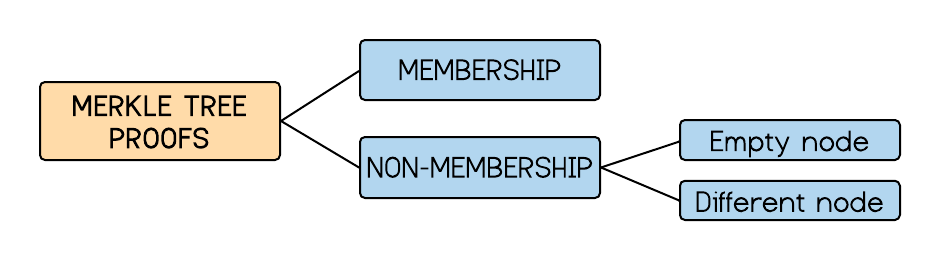
\includegraphics[scale=0.8]{MT-pfs-h.png} 
%	  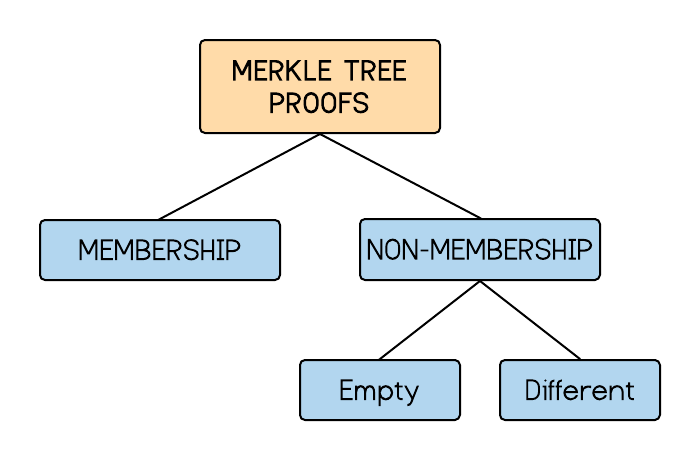
\includegraphics[scale=0.8]{MT-pfs.png} 
\end{figure}
% https://www.lucidchart.com/documents/edit/f1bfd196-fbcf-4934-b3cd-91fb0d057f32/0

%\begin{tikzpicture}
%\draw[->] (0,0) -- (2,0.5) node[pos=.5,sloped,above] {$x$};
%\draw[->] (0,0) -- (2,-.5)  node[pos=.5,sloped,below] {$y$};
%\end{tikzpicture}

% Definició dels possibles nodes (fulla, buit, diferent i nodes interns)

%\begin{centering}
%Merkle Tree Proof
%\begin{itemize}
%	\item Membership
%	\item Nonmembership
%		\begin{itemize}
%			\item Empty node
%			\item Different node
%		\end{itemize}
%\end{itemize}
%\end{centering}
%\begin{tikzpicture}[auto,node distance=1.5cm]
%  % Create an entity with ID node1, label "Fancy Node 1".
%  % Default for children (ie. attributes) is to be a tree "growing up"
%  % and having a distance of 3cm.
%  %
%  % 2 of these attributes do so, the 3rd's positioning is overridden.
%\node[draw] (a) {Merkle Tree Proof}
%    [grow=right,sibling distance=3cm]
%    child { node[draw, pos=.5,sloped,above] (b) {Nonmembership}
%    		child {node[draw] (d) {Empty node}}
%		child {node[draw] (e) {Different node}}
%	  }
%    child {node[draw, pos=.5,sloped,below] (c) {Membership}};
%\end{tikzpicture}

%\subsection{Diagram}

%\begin{tikzpicture}[auto,node distance=1.5cm]
% \node [draw] (r){ root }
%  child { node [draw]  (a) { } % fill
%    		child {node [draw] (c) { }}
%    		child {node [draw] (d) { }}
%  	}
%  child { node [draw] (b) { }
%    		%child {node [empty] (e) { }}
%    		%child {node [leaf] (f) { }}
%  	};
%\end{tikzpicture}

Dibuixet. 
